\documentclass[11pt]{article}

\usepackage[utf8]{inputenc}
\usepackage[T1]{fontenc}

\usepackage[a4paper, left=2cm, right=2cm, top=3.5cm, bottom=3.5cm]{geometry}
\usepackage[french]{babel}

% Paragraph spacing
\setlength{\parskip}{1em}

% Fancy headers
\usepackage{fancyhdr}

% Captions for subfigures
\usepackage{subcaption}


% Code highlighting
\usepackage{minted}

% Footnote inside a caption
\usepackage{fnpos}
\usepackage{ftnxtra}

% Maths
\usepackage{amsmath}
\usepackage{amssymb}

% Todo notes
\usepackage{todonotes}

% Table of contents for bibliography
\usepackage[nottoc]{tocbibind}

% Inline monospace font
\def\code#1{\texttt{#1}}

% Figures
\usepackage{graphicx}

% Draw figures
\usepackage{tikz}

% Code listing
\usepackage{listings}

% Tikz node rotation
\usetikzlibrary{positioning}

% Turing machine
\usetikzlibrary{chains,fit,shapes}

% Usage: \rotnode[options]{rotation}{text}
\newcommand\rotnode[3][]{%
\node [#1, opacity=0.0] (tmp) {#3};
\node [draw, rotate around={#2:(tmp.center)}] at (tmp) {#3};
}

% Clickable links
\usepackage{hyperref}
% Table of contents depth
\setcounter{tocdepth}{2}

% Inline code
\usepackage{listings}
\usepackage{color}

\title{Systèmes d'exploitation}

\author{William SCHMITT \& Othmane AJDOR}
\date{2018-2019}

\begin{document}
\maketitle

\section{Introduction}
\subsection{Bibliographie}

Tanenbaum: Modern Operating Systems \\
Silberschatz: Operating Systems Concepts

\subsection{Plan}

\paragraph{Cours/TD}
\begin{itemize}
	\item Moniteurs
	\item Sémaphores
	\item futex
\end{itemize}

\paragraph{TP (pas à rendre)}
\begin{itemize}
	\item 1ère période : rappels de C
	\item 2ème période : mmap
\end{itemize}

\paragraph{TP (à rendre)}
\begin{itemize}
	\item Allocateur mémoire virtuel (malloc) : révisions sur les pointeurs
	\item Shell (fork, exec, redirection IO)
	\item Thread (lecteur vidéo multithread)
\end{itemize}

\paragraph{Présentation scientifique :} article de usenix.org (de 2019, 2018 ou dans les \textit{best papers} des 3 dernières années) à présenter devant la classe.

\subsection{Examen}
\begin{itemize}
	\item QCM: 1h (20 à 25 questions) \\
	\item TP:
	      \begin{itemize}
		      \item 2h (75\%)
		      \item Présentation scientifique (25\%)
	      \end{itemize}
\end{itemize}


Notation : 50/50.

\subsection{Fibonacci}
Comparaison avec/sans printf, ratio de performance : 397

Avec redirection de stdout dans /dev/null, le ratio plonge à 31.

Lorsque les tampons sont pleins (dans le terminal), on bloque les producteurs de données le temps de vider les tampons (et donc d'afficher les résultats).

Facteurs décorrélés de l'algorithme permettant des gains :
\begin{itemize}
	\item IO
	\item Gestion de la mémoire
\end{itemize}

\section{Hardware}
On se base sur un modèle simpliste.
\begin{figure}
	\centering
	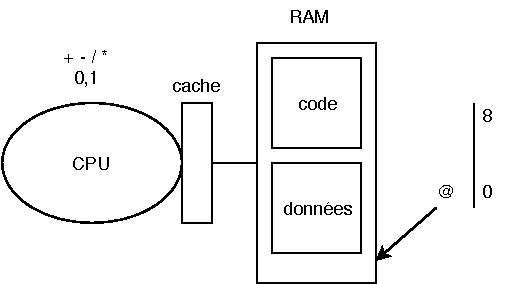
\includegraphics{img/cpu+ram.pdf}
\end{figure}

Depuis les années 1990, la vitesse du CPU a dépassé celle de la mémoire. En un cycle CPU (pour un CPU à 4GHz), un photon peut parcourir 7,5cm. On rajoute à cette époque du cache dans les CPU pour compenser la lenteur de la mémoire.

De plus, la taille de la mémoire a explosé.

\section{Système d'exploitation}
Dans les premier ordinateurs, on réglait l'état mémoire à la main avec des interrupteurs.

\begin{figure}
	\centering
	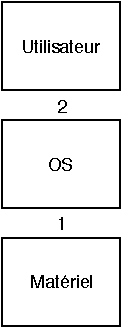
\includegraphics{img/hw-os-user.pdf}
\end{figure}

Un OS est à la base composé de différentes routines qui ont deux buts :
\begin{enumerate}
	\item Gestion du matériel (partage, arbitrage, partition, droits/utilisateurs) \begin{itemize}
		      \item Processeurs (dont la complexité augmente)
		      \item Disques/SSD/Burst buffer/Bandes magnétiques
		      \item RAM
		      \item Interfaces réseau
	      \end{itemize}
	\item Abstractions
	      \begin{itemize}
		      \item Fichiers, répertoires, systèmes de fichiers
		      \item processus
		      \item utilisateurs
		      \item socket réseau
	      \end{itemize}
\end{enumerate}

\subsection{Composition d'un OS}
Le noyau Linux est constitué d'environ 18 millions de lignes en C. Ingérable par une seule personne, il est décomposé en modules exposant des API puis compilé en un programme comme les autres, à quelques exceptions près.

\paragraph{Mode d'exécution} un OS s'exécute dans un mode spécial et a accès à des instructions spéciales.

\paragraph{Interruptions et exceptions} permettent de passer du mode user au mode kernel. La différence entre les deux : les interruptions sont masquables.

\paragraph{Bibliothèque système côté utilisateur} permettant (notamment) d'éviter de coder les interruptions à la main.

S'il s'agit d'un programme comme les autres : où et quand est-il en RAM ? Où et quand s'exécute-t-il ?

Il est toujours en RAM (notamment pour pouvoir répondre aux interruptions), avec certaines nuances : tout l'OS n'est pas en mémoire ! Pour Linux, seuls certains modules sont chargés, notamment pour des drivers. Sous Windows, les parties non utilisées sont sur disque (swap).

En termes d'exécution, il n'est exécuté que lors d'interruptions/exceptions.

Déroulement du boot
\begin{itemize}
	\item Intel ME (management engine), codé sur le processeur et peut faire tourner Minix.
	\item BIOS/UEFI : exécuté directement par le CPU au boot, accessible comme de la mémoire normale, pour chercher le chargeur et le mettre en mémoire. Fourni par le fabricant de mobo, il y a déjà des interactions avec le matériel avant le chargement de l'OS. L'accroissement de complexité de l'UEFI (possibilité de surfer) présente des problématiques de sécurité.
	\item Chargeur : mise en RAM des données sur disque \begin{itemize}
		      \item Windows
		      \item GRUB
		      \item Autre...
	      \end{itemize}
	\item Initialisation
	\item Vecteurs d'interruption/exception
\end{itemize}

La maîtrise de la machine physique devient de plus en plus lointaine, même au niveau des OS.

\subsection{Modularité}
\begin{figure}[h!]
	\centering
	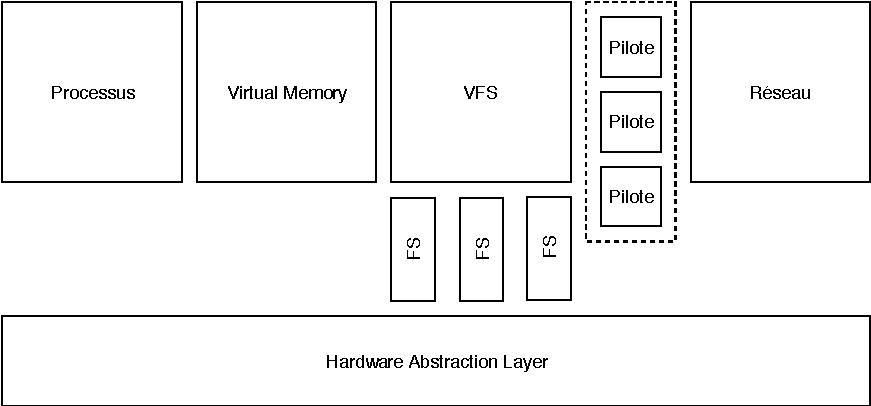
\includegraphics{img/modular-os.pdf}
\end{figure}

% \pagebreak

\subsection{Plan du cours}
\begin{itemize}
	\item Processus / Threads
	\item Synchronisation / prog concurrente
	\item Ordonnancement (Théorie+pratique)
	\item Mémoire -> coté user
	\item Pagination, mémoire virtuelle
	\item FileSystem (période 6)
	\item Sysd (intro)
	\item Multi Proc (programmation OpenMP)
\end{itemize}

Les \textbf{systèmes de fichier virtuels} sont une API haut niveau pour l'ouverture, la fermeture, la lecture, l'écriture de fichiers. Les filesystems sont par exemple ext4, btrfs, fat, fat32, ntfs.

\section{Histoire}
"L'histoire de l'informatique, ça remonte aux machines automatiques pour faire des trucs."
\subsection{Préhistoire}
\begin{itemize}
	\item Babylone
	\item Machine Héron d'Alexandrie
\end{itemize}

\subsection{Histoire}
\paragraph{Epoque mécanique}
\begin{itemize}
	\item Pascal
	\item Babbage: machine universelle programmable
	\item Ada Lovelace (if, boucle)
\end{itemize}

\paragraph{Antiquité}
\begin{itemize}
	\item Turing
	\item ENIAC
\end{itemize}

\paragraph{Moyen-Âge}
\begin{itemize}
	\item IO: cartes perforées
	\item Tampon: copie des IO en RAM
\end{itemize}

\paragraph{Monde moderne (1960)}
\begin{itemize}
	\item MULTICS: OS moderned (processus, droits, fichiers, multi-utilisateurs)
	\item 1969 : Mini-ordinateur: PDP11
	\item UNIX : (asm pour la première version, C pour la deuxième)
	\item 1974 : Micro-ordinateurs
	      \begin{itemize}
		      \item Grand public : pas assez puissants pour faire tourner UNIX, donc utilisation de CP/M (8 bits, 16ko RAM) puis DOS en 1981
		      \item Station de travail : permettent de faire tourner UNIX
	      \end{itemize}
	\item 1987 : Minix, reste petit pour permettre d'être un outil pédagogique (bouquin avec src + explication)
	\item 1991 : Linux \begin{itemize}
		      \item internet
		      \item GPL : possibilité de voir et modifier le code, obligation de distribuer le code modifié
	      \end{itemize}

\end{itemize}

\subsection{1990-}
\begin{itemize}
	\item Linux (1991)
	\item Internet
	\item GPL libre (source, modification, reverser)
\end{itemize}

\pagebreak

\section{Processus}
\subsection{Activités parallèles}
\begin{itemize}
	\item materiel
	\item abstraite: logiciel, utilisateurs
	\item competition (tout ce qui n'est pas partageable ei: entrée RAM)
	\item cooperation (coexistence de deux programmes qui doivent tourner en meme temps)
\end{itemize}

Pour gérer cela, il faut des programme\textbf{\underline{S}}\\
-> séparation des activités\\
-> cohabitation des données et programmes\\
Utilisation de mémoire virtuelles au lieu de celles physiques.\\
Indirection dans les adresses manipulées par les programmes.

\begin{lstlisting}[frame=single]  
    int a; // juste la somme de la taille
    const in b = 10; // read only
    int c = 20;
    int main(integer c, char **argv){
        int *d = malloc(atoi(argv[1])); // allocation dynamique de 20 oct
        free(d);
        return 0;
    }
    
\end{lstlisting}

Pagination: espace virtuel est coupé en page de 4ko pour n'avoir que les morceaux intéressants de la mémoire

\subsection{Processus}
\subsubsection{Quantum}
\begin{itemize}
	\item Partage de plusieurs processus (\~1000) (peu de coeurs/processeurs)
	\item Partage du temps CPU en tranche (quantum)
	\item Horloge -> interruption -> traitant -> context\_switch -> fin traitant restauration -> retour d'interruption restauration minimal
	\item I/O
	\item terminaison
	\item Synchronisation
	\item sleep
\end{itemize}
\pagebreak
\subsubsection{Contexte d'un processus}
\begin{itemize}
	\item code -> RAM
	\item données -> RAM + registres du processeur | sauvegarde restauration
	\item instructions i1 \textbf{|} i2
\end{itemize}

\subsubsection{Processus}

\paragraph{Processus}
Espace de mémoire (virtuelle/privée) + 1 programme (données)
\paragraph{Threads connus par l'OS}
partie executive d'un processus, execute \underline{\textit{1}} fonction
\paragraph{Threads user connus par le programme}
(fiber, task, co-routine, go-routine...)

\subsubsection{Scheduler / Ordonnanceur}
Fonction qui choisit le prochain élu à partie d'une liste (structure de données centrale par l'OS) de processus prêts.\\
Le scheduler est exécuté à chaque changement de processus.

\begin{figure}[h!]
	\centering
	%\includegraphics{img/automate-scheduler.pdf}
\end{figure}

\pagebreak

\section{Virtualisation}
\subsection{Niveaux de virtualisation}
\subsubsection{Hardware}
\begin{itemize}

	\item mainframe IBM: fait tourner des OS où chacun croit être le seul sur la machine
	\item Intel (peut faire pareil, marche +/- bien) -> Xen\\
	      4 mode de protection du CPU (3 user à 0 kernel), mode -1 permet de changer la position de l'indice PC, qui normalement ne peut pas être changée.
\end{itemize}

\subsubsection{OS}
\paragraph{VM}
VirtualBox, Qemu ...où l'OS hôte fait tourner des OS invités
KVM permet de mettre des instructions de l'OS invité sur le matériel de l'OS hôte.
\paragraph{Container}
Container Docker, on ne simule pas un OS complet au dessus d'un autre, mais on va par exemple séparer le Filesystem, le réseau, allouer la RAM différemment. Il existe un seul OS dans ce cas mais certaines bibliothèques peuvent être rendues privées pour un conteneur mais pas pour l'autre.
\paragraph{JAVA -> JVM}
Java compile le code en instruction assembleur qui seront exécutées sur une JVM qui tourne sur l'OS. Python et Perl font à peu près la même chose (JiT).

\subsubsection{Sondage Partage Processus/Thread}
% \paragraph{Programme}
% Processus 1 -> Thread 1 (une fonction du programme du processus)
% \paragraph{Pile}
% 1 par Thread du processus, soit plusieurs <- 1 par Thread
% \paragraph{Données}
% \paragraph{Fichiers}

\begin{table}[h!]
	\begin{tabular}{l|l|l|}
		\cline{2-3}
		                                                                 & Processus                        & Threads                                   \\ \hline
		\multicolumn{1}{|l|}{code}                                       & 1                                & 1 fonction du code                        \\ \hline
		\multicolumn{1}{|l|}{pile (variables locales)}                   & autant que de threads            & 1 par thread                              \\ \hline
		\multicolumn{1}{|l|}{fichiers (open, close, read, write)}        & descripteurs de fichiers ouverts & \multicolumn{1}{c|}{\_\_\_\_\_\_\_\_\_\_} \\ \hline
		\multicolumn{1}{|l|}{réseaux (comme les fichiers)}               &                                  &                                           \\ \hline
		\multicolumn{1}{|l|}{exit (terminer un processus)}               &                                  &                                           \\ \hline
		\multicolumn{1}{|l|}{données (variables globales/comme le code)} &                                  &                                           \\ \hline
	\end{tabular}
\end{table}

\pagebreak

\section{Processus sous UNIX}
\subsection{Outils}
\begin{itemize}
	\item ps,
	      htop,
	      top,
	      px,
	      pstree
	\item taille en mémoire, taille complète (mais la plupart des données sont inutiles)
	\item taille en RAM (trompeur comme plusieurs portions de la mémoire sont partagées, e.i: libc, printf, malloc...). Smem pour donner des info
	\item OOM\_Killer -> tue le + gros (mais pas X11 quand meme)
\end{itemize}

\subsection{Fork}
\begin{lstlisting}[frame=single]
int r = fork(); // cree une copie du processus appelant  
switch(r){
	case -1:
		perror("mon fork:"); //mon fork:not enough memory ou autre
		break;
	case 0:
		lefils
		break;
	default:
		le pere de "r" (PID de mon fils)
}  
\end{lstlisting}

Après l'appel de fork, le processus fils continue ce qu'on père était en train de faire.

\subsection{exec}
exec [p|up|lp|le|e]
\begin{lstlisting}[frame=single]
	execvp("file", tab);
	// arg1: nom programme apres lancement, arg2: nom commande,
	// arg3: parametres de la commande lancee
	execlp("ls", "ls", "-l"); 
\end{lstlisting}

\subsection{Wait}
wait(), waitpid() (exclusivité du père), attend la mort du processus

Lors du lancement de ls -R /, le shell attend la fin du ls avant de refaire un prompt.
Si on utilise ls -r / \textbf{\&}, le shell n'attend pas

\subsection{Signal}
kill(pid, SIGNumber)\\
kill -9 -1, tuer tous les processus brutalement, meme le shell
kill -15 -1, tue plus gentillement, les applis ont le temps

\pagebreak

\section{Threads}
\subsection{Création d'un thread}

\begin{lstlisting}[frame=single]
	int main(){
		auto th = new thread([](){cout << "hello" << endl;});
		th->join();
	}	
\end{lstlisting}

\subsection{Gestion de la concurrence}
Variables d'états \underline{partagées}
Stratégie: modification 1 à la fois
\begin{itemize}
	\item instructions atomiques (couteuses, marchent 1 mot à la fois soit <- très localisé)\\
\end{itemize}

Exemple de base: 2 threads executant A() et B(): le but est d'afficher 20
\begin{lstlisting}[frame=single]
	int a = 10;
	A(){
		a=20;
	}
	B(){
		printf("%d\n", a);
	}
\end{lstlisting}
Ne marche pas

\begin{lstlisting}[frame=single]
	int a = 10;
	bool fini = false;
	A(){
		a=20;
		fini=true;
	}
	B(){
		while(!fini);
		printf("%d\n", a);
	}
\end{lstlisting}
Ne marche toujours pas

\pagebreak


Tony Hoare, le meme gars qui a inventé le qsort, a proposé l'utilisation de monitors, des fonctions en exclusion mutuelle. \\
On utilise aussi des variables de condition, elles servent à attendre jusqu'à ce qu'on nous reveille (wait, signal).

\begin{lstlisting}[frame=single]
	mtx_t m; // mutex
	cnd_c c;
	int a = 10;
	bool fini = false;
	A(){
		mtx_lock(&m);
		a=20;
		fini=true;
		mtx_unlock(&m);
	}
	B(){
		mtx_lock(&m);
		while(!fini); // attente active (c'est mal !) (energie)
			// auto[unlock au wait | lock au reveil] sur m
			cnd_wait(&c, &m) 
		printf("...")
	}
\end{lstlisting}

\pagebreak

\section{TD1 - Dekker}
Avec deux processeurs:
\begin{lstlisting}[frame=single]
	debut_SCC();
		load $i, %r0
		inc %r0
		store %r0, $i
	fin_SCC();
\end{lstlisting}
Après l'execution des instructions, i=1|2.\\
Ce qu'on veut avoir c'est obtenir i=2 et pas i=1

\subsection{Zero}
En utilisant cette fonction:
\begin{lstlisting}[frame=single]
	bool occ=false; //occupe
	debut_SCC(){
		alpha: 
			if (occ) 
				goto alpha; 
			occ = true;
	}

	finSCC(){
		occ = false;;
	}
\end{lstlisting}
On n'obtient pas d'exclusion mutuelle.

\pagebreak

\subsection{One}
\begin{lstlisting}[frame=single]
	bool occ = false;
	\\ecrire avant le test
	
	debut_SCC(){
		int old = occ; // local var
		occ = true;
		alpha : if(old)
					old = occ;
				goto alpha;
	}

	finSCC(){
		occ = false;
	}
\end{lstlisting}
Pas d'exclusion mutuelle.

\subsection{Two}
\begin{lstlisting}[frame=single]
	int tour = 0;
	p; // num de processeur {0;1}
	q = 1 - p; // num de l'autre processeur

	debut_SCC(){
		alpha:
			if (tour != p){
				goto alpha;
			}
	}

	finSCC(){
		tour = 1 - p;
	}
\end{lstlisting}
Exclusion mutuelle OK, par contre, le bout de code cause un problème de famine.\\
L'autre processeur ne pourra jamais executer la section critique.

\pagebreak

\subsection{Three}
\begin{lstlisting}[frame=single]
	bool access[2] = {false};
	//Accede a acces[] avec p/q <-annoncer ma demande avant la boucle 

	debut_SCC(){
		acces[p] = true;
		alpha:
			if (acces[q])
				goto alpha;
	}

	finSCC(){
		acces[p] = false;
	}
\end{lstlisting}
Exclusion mutuelle OK.\\
Si les deux processeurs executent le code en même temps, ils rentrent dans une boucle infinie.\\
Probleme de \textbf{dead\_lock}, les deux processeurs ne font plus rien.

\subsection{Four}
\begin{lstlisting}[frame=single]
	bool access[2] = {false, false};
	// Three et renoncer a sa demande
	// On recommence tout

	debut_SCC(){
		alpha:
			acces[p] = true;
			if (acces[q])
				acces[p] = false;
				// en reseau recursive doubling
				sleep(random); 
				goto alpha;
	}

	finSCC(){
		acces[p] = false;
	}
\end{lstlisting}
Probleme de \textbf{dead\_lock} si synchrone
Il faut qu'ils arrivent en même temps et qu'ils restent synchrones pour que ça marche.

\pagebreak

\subsection{Five}

\begin{lstlisting}[frame=single]
	bool access[2] = {false, false};
	int tour;
	// Comme la Four
	// Celui dont ce n'est pas le tour renonce

	debut_SCC(){
		alpha:
			acces[p] = true;
			if (p != tour && acces [q])
				acces[p] = false;
				sleep(random); 
				goto alpha;
	}

	finSCC(){
		acces[p] = false;
		tour = q;
	}
\end{lstlisting}
Pas d'exclusion mutuelle

\pagebreak

\subsection{Six}

\begin{lstlisting}[frame=single]
	bool access[2] = {false, false};
	int tour;
	// Comme la Four
	// Celui dont ce n'est pas le tour renonce

	debut_SCC(){
		acces[p] = true;
		
		alpha:
			if(acces[q]){
				if(tour==p){
					beta:
						if(access[q])
							goto beta;
				}
				else {
					acces[p] = false
					sigma: if(tour==q):
						goto sigma;
					goto alpha;
				}
			}

		}

	finSCC(){
		acces[p] = false;
		tour = q;
	}
\end{lstlisting}
Avant de commencer, je verifie que je suis dans le bon etat.\\
Meme si c'est mon tour, je vais attendre que l'autre renonce à acces.\\
L'autre cas c'est si je suis en conflit, je renonce à mon tour.\\
Une fois qu'il a fini, le tour devriendra le miens

\pagebreak

\subsection{Seven - La solution correcte de Peterson}
La solution correcte:
\begin{lstlisting}[frame=single]
	bool access[2] = {false, false};
	int dernier;

	debut_SCC(){
		acces[p] = true;
		dernier = p;
		alpha:
			if (acces[q]){
				if(dernier ==p)
					goto alpha;
			}

	finSCC(){
		acces[p] = false;
	}

\end{lstlisting}
\end{document}